\subsection{Laptop}
\label{subsec:laptop}

The reasons I choose Typescript for the Laptop-side software are that this is the language I have the most experience with and that, when used in the context of a webapp, it facilitates easy visualization of data.
This is especially helpful for debugging, but comes at the price of performance, which I assume is lower than what can be achieved with other languages such as C.

\paragraph{Proxy}
Because a webapp cannot directly access the serial port, I wrote a proxy script, which reads from the serial port and provides received data via the WebSocket protocol.

\paragraph{Detecting a Rotation}
Detection of a $180\deg$ rotation from left to right is implemented via a state machine. The states can be seen in Figure \ref{fig:stateMachine}.
The relevant sensor values for this detection is the X value of the gyroscope on the MPU6050.
Because the values are not 0 even when the board is completely still, I decided to use the first 50 received values for calibration.
This means that the board should be stable for the first about 2 seconds (see chapter \ref{subsec:benchmark}) after connection with the laptop is established.
Those values are used to calculate mean and standard deviation.

If a received value is within $x$ times the standard deviation of the mean, the platform is considered to not be turning.
If the value is above or below the threshold, the state machine goes to the $Over$/$Under$ states respectively.
While in the $Over$/$Under$ states, a counter is maintained, which is increased for each measurement outside the threshold and decreased if the platform is stable again.
If the counter reaches 0, the state returns to the standard, i.e. $Steady$. If the counter reaches a threshold, the state changes to $Over\_Steady$ or $Under\_Steady$ depending on previous state.
While these additional states are not currently utilized, they allow to further customize the detection behavior.

While in the $Over$ or $Over\_Steady$ states, if value significantly under mean is detected, state is instantly reverted back to $Steady$ and the current rotation ends. Same thing happens for values significantly over mean while in $Under$ or $Under\_Steady$ state

Start of rotation is therefore detected when the state changes away from $Steady$ and end of rotation upon returning to $Steady$.
For detecting the length of rotation, the sensor values are summed up while state is not $Steady$.
After a rotation ends, this value can be compared against thresholds to determine what direction this turn was (corresponds to the sign of the sum) and how big the turn was (corresponds to the absolute value of the sum).
Given the known frequency and sensitivity of the sensor, this sum can also easily be turned into an estimate of distance of rotation, see Equation \ref{eq:angle}. For this project, range is 250, since the sensor is configured to use the $\pm50\deg\\s$ range. Frequency was determined to be 31.5, see \ref{subsec:benchmark}.

\begin{equation}
    (sum * range) / (2 ^{15}  * frequency)
    \label{eq:angle}
\end{equation}

\begin{figure}
    \centering
    \includegraphics[width=\linewidth]{figures/stateMachine.pdf}
    \caption{States of the turn classification}

    \label{fig:stateMachine}
\end{figure}

\paragraph{Capturing Ultrasound Data}
Every reading of the ultrasonic reading that comes in while the device is in rotation is saved together with the current angle of rotation, i.e. the sum of gyroscope readings. Additionally, a buffer is kept to include the last n (5) values once the start of a turn is recognized.

\paragraph{Normalizing Data}
Due in part to the variable update rate, which is discussed in Section \ref{subsec:benchmark}, the captured readings need to be normalized.
This is done by using the sum of gyroscope readings starting from the beginning of rotation as x-coordinate for the current distance reading.
The total sum of gyroscope readings for a rotation then corresponds to $180\deg$ and other values can be scaled accordingly.
While the gyroscope readings give a speed of rotation rather than a distance, a Sum should still work given the very steady frequency of updates from the MPU (see chapter \ref{subsec:benchmark}).
For distance of rotation would be speed of rotation multiplied by time, if we have constant time a simple sum should suffice.
Distances are also scaled to a range between 0 and 1 for the shortest and longest measured distance respectively.

% TODO: describe problem with graphing environment

\paragraph{Evaluating Data}
Once the end of a turn is registered by the state machine, we have all the data necessary to evaluate the junction at hand.
Classification happens by comparing the List of ${x,y}$ objects, where $x$ is the normalized angle and $y$ the normalized distance, to known profiles of T-Junctions, X-Junctions and Corridors.

For this, the data is converted to a discrete array. For every integer x from 0 to 180, all data points are collected whose angle starts with x. Then, the average of their distance measurement is calculated. This leaves us with a list of up to 180 numbers, as not every angle may have been recorded. We now calculate the correlation between this series and a series of reference value for each of the junction types, where missing data in either series is removed from both.

This leaves us with correlation values for each junction type and we can return a list of junction types sorted by how likely this type is to correspond with our observation. This means that the first value in the returned list is the best fit and therefore our evaluation result.

For the reference data, I first wanted to use theoretically computed data, as can be seen in Figure \ref{fig:theory}, however this did not work well.
Therefore I decided to use empiric data created by adding measurements from several scans together and normalizing them. The resulting data can be seen in Figure \ref{fig:actual}.

A different approach I tried but decided to discard in favor of the approach described above used KMeans clustering.
One of the benefits was the vastly reduced amount of data that needed to be saved.
The idea was to generate 5 clusters from the scanned data via KMeans. The center of these Clusters could then be compared to the center of the clusters for the reference data.
Thus for each of the three reference classes only the center of the five clusters would need to be saved, instead of the 180 data points.
However, this did not work reliably.
Maybe this approach could be used in the future, if clusters are calculated multiple times and distances are then combined.

Regardless of classification method is used, upon classifying the Junction the webapp adds a new chart to the page that includes the classification result and plots the normalized data.

\begin{figure}
    \centering
    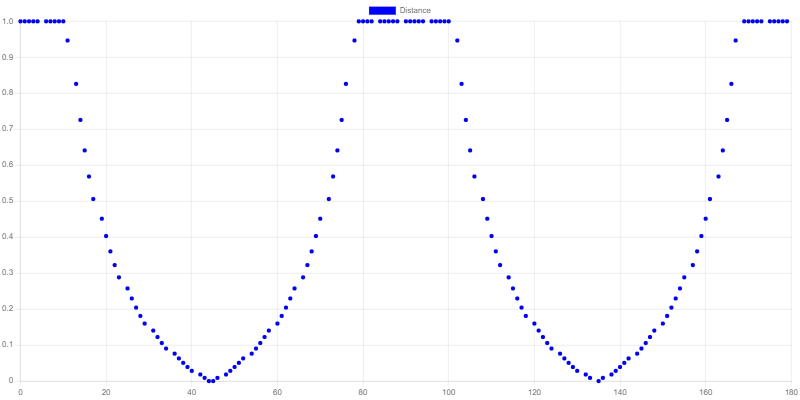
\includegraphics[width=0.45\linewidth]{figures/x_graph.png}
    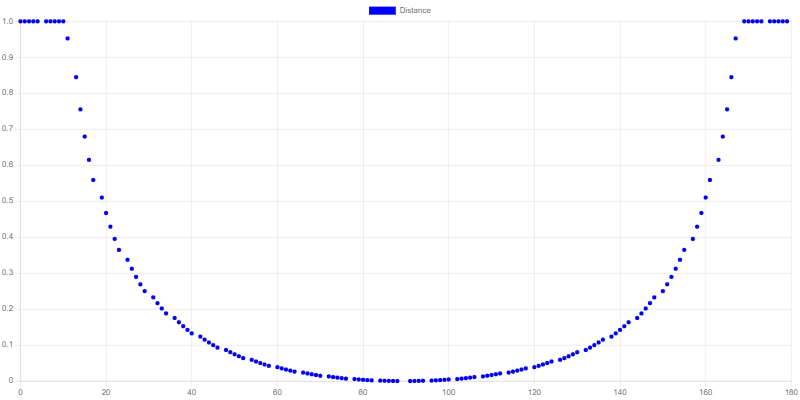
\includegraphics[width=0.45\linewidth]{figures/t_graph.png}
    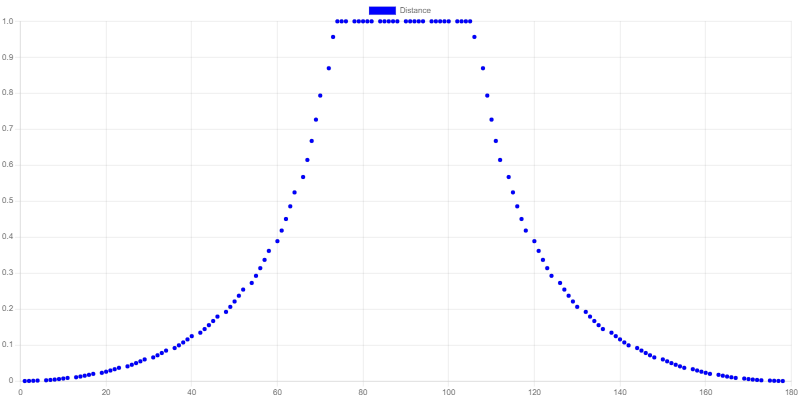
\includegraphics[width=0.45\linewidth]{figures/c_graph.png}
    \caption{Expected Scan data for X-Junction, T-Junction and Corridor}

    \label{fig:theory}
\end{figure}

\begin{figure}
    \centering
    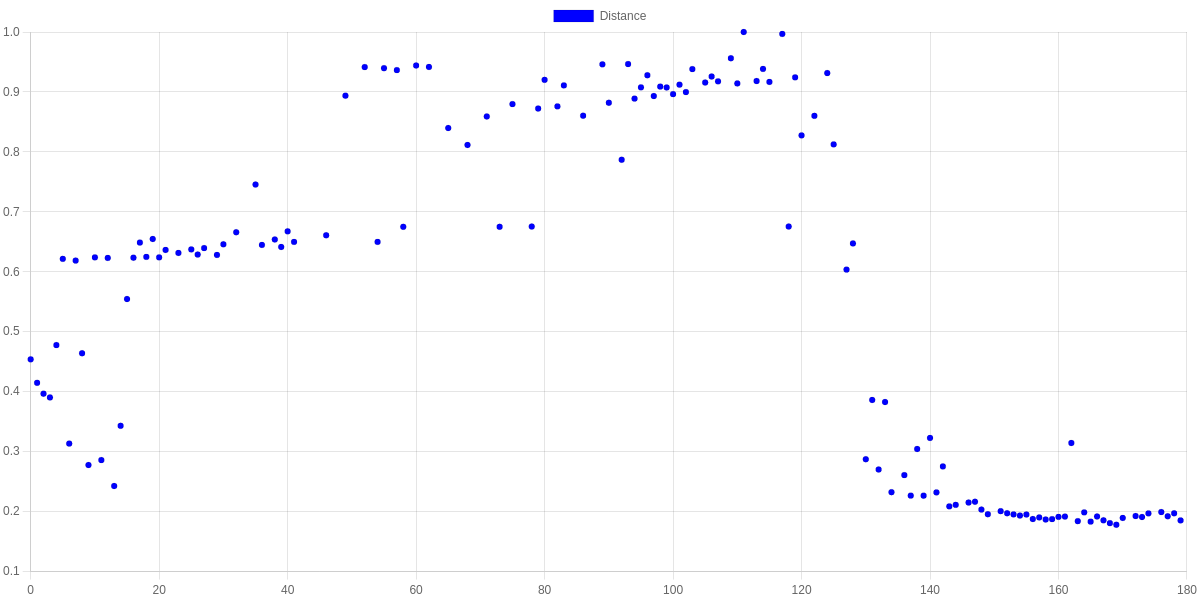
\includegraphics[width=0.45\linewidth]{figures/x_graph_empiric.png}
    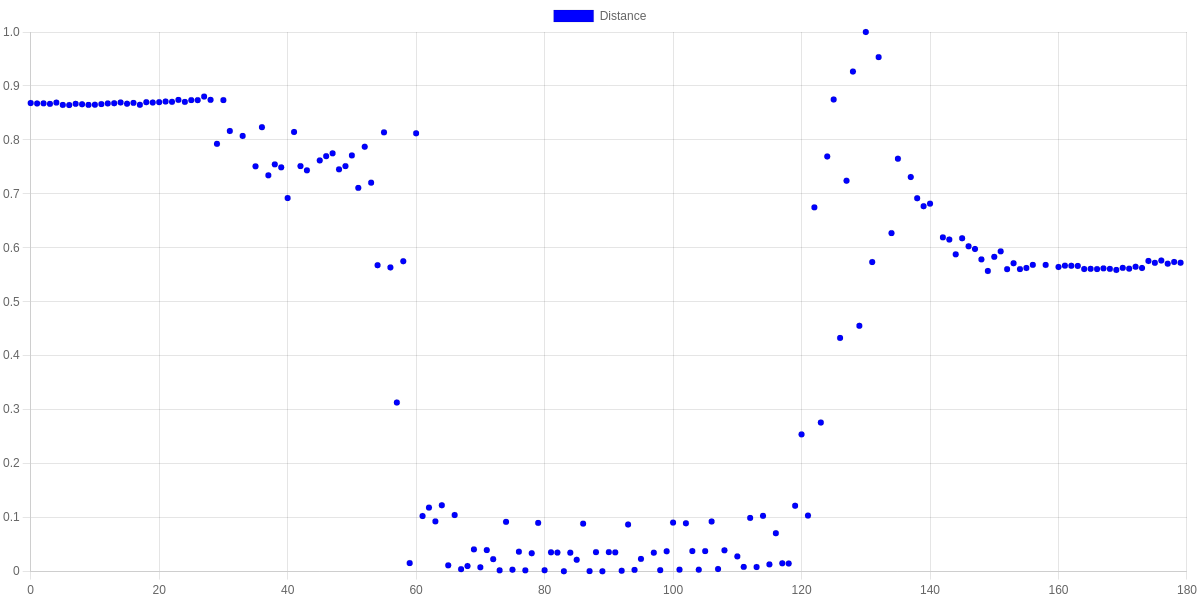
\includegraphics[width=0.45\linewidth]{figures/t_graph_empiric.png}
    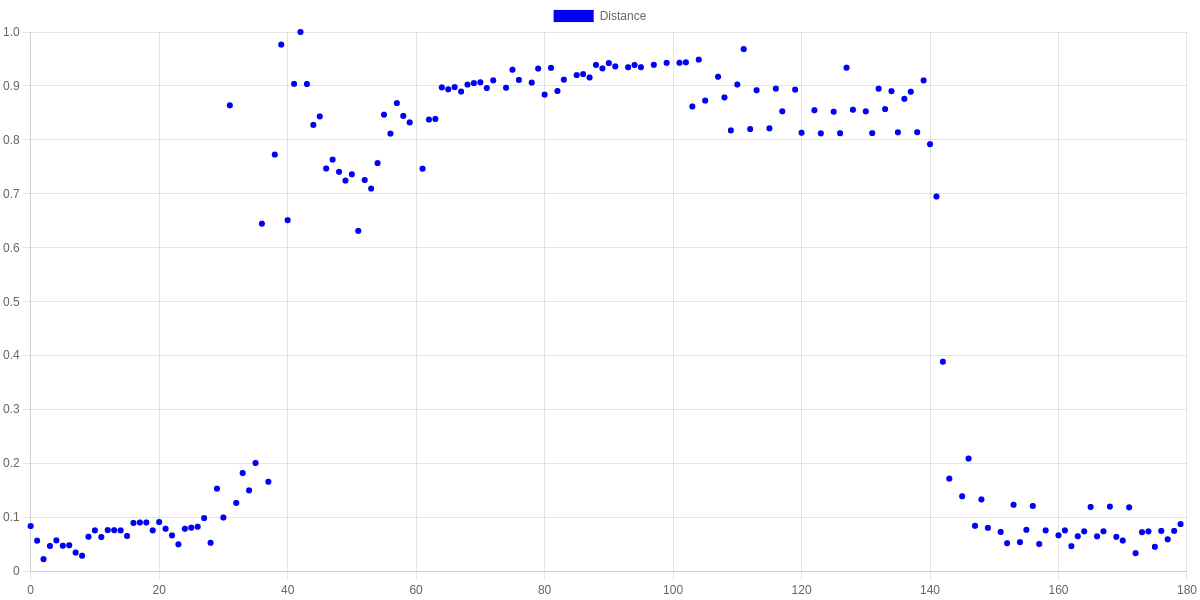
\includegraphics[width=0.45\linewidth]{figures/c_graph_empiric.png}
    \caption{Empiric data for X-Junction, T-Junction and Corridor.
        Mixture of several scans, used as reference in classification}

    \label{fig:actual}
\end{figure}

\paragraph{Extensibility}
The code can easily be modified to include different handlers for the sensor data.
The best place for this is the switch statement in the main.ts file, where the prefix is used to differentiate between sensor types.
For example, the code includes a function that can be used to live-plot values as soon as they arrive.